\documentclass[hyperref={pdfpagelabels=false}]{beamer}
\usepackage{lmodern}
\usepackage[utf8]{inputenc}
\usepackage{amssymb}
\usepackage{amsmath}
\usepackage{tikz}
\usepackage{tkz-euclide}
\usepackage[percent]{overpic}
\graphicspath{{Pictures/}}
\usetikzlibrary{arrows,calc,intersections,shapes,backgrounds,shadows,automata}
\usetheme{Berlin}
\definecolor{UniRed}{RGB}{255,0,0}
\definecolor{UniWhite}{RGB}{255,255,255}
\definecolor{PresiBlue}{RGB}{50,57,171}
\setbeamercolor{eecks} {bg=UniRed, fg=UniWhite}
\setbeamercolor{presinative}{bg=PresiBlue, fg=UniWhite}

% Layer tikz definitions
\tikzstyle{block} = [
	rectangle, draw, fill=blue!20, 
	text width=20em, text centered, 
	rounded corners, minimum height=4em,
	node distance=2.5cm]

\tikzstyle{block-active} = [
	rectangle, draw, fill=green!20, 
	text width=20em, text centered, 
	rounded corners, minimum height=4em,
	node distance=2.5cm]

\tikzstyle{cloud} = [draw, ellipse,fill=red!20, node distance=2cm, minimum height=2em]

\tikzstyle{line} = [draw, ->, >=stealth', ultra thick]
\tikzstyle{dline} = [draw, <->, >=stealth', ultra thick]

% Router tikz definitions
\def\robot at (#1,#2) {
	\draw[fill=red] (#1,#2) circle (0.35);
	\draw[fill=blue] (#1,#2)++(0.15,0) circle (0.1);
}
\def\goal at (#1,#2) {
	\draw[red,line width=8pt] (#1,#2)+(-.35,-.35)--+(.35,.35) +(-0.35,0.35)--+(.35,-.35);
}
\def\goalHelp at (#1,#2) {
	\draw[green!80!blue,line width=8pt] (#1,#2)+(-.35,-.35)--+(.35,.35) +(-0.35,0.35)--+(.35,-.35);
}
\tikzstyle{edge} = [draw,line width=24pt,-,gray]
\tikzstyle{selected edge} = [draw,line width=24pt,-,green]
\tikzstyle{ignored edge} = [draw,line width=24pt,-,red!50!white]
\tikzstyle{obstacle} = [draw,very thick,circle,minimum size=20pt,shading=radial,outer color=black!80!white,inner color=white]
\tikzstyle{selected obstacle} = [draw,very thick,circle,fill=blue!20!white,minimum size=20pt]

% Title
\title{\textsc{RoboSoccer} Project Plan}  
\author[Hofbauer, Jiang, Meyer, Schmidt, Wirnshofer]{
  Markus~Hofbauer \and
  He~Jiang \and
  Kevin~Meyer \and
  Benedikt~Schmidt \and
  Florian~Wirnshofer
}
\institute
{
	Technische Universit\"at M\"unchen, Germany
}
\date{June 4, 2014}

% Presentation
\begin{document}
\begin{frame}
	\titlepage
\end{frame} 

\begin{frame}
	\frametitle{Table of contents}
	\tableofcontents
\end{frame} 

\section{Introduction} 
\begin{frame}
	\frametitle{Introduction} 
\end{frame}

\section{Class Diagram}
\begin{frame}
	\frametitle{Layers}
	\begin{center}
		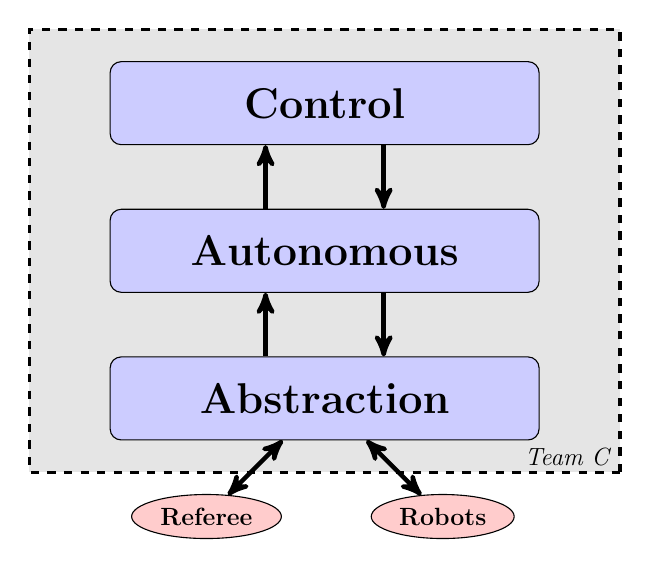
\begin{tikzpicture}[scale=0.75, transform shape]		
		    % Layers
			\node [block] (control) {\huge \textbf{Control}};
		    \node [block, below of=control] (autonomous) {\huge \textbf{Autonomous}};
			\node [block, below of=autonomous] (abstraction) {\huge \textbf{Abstraction}};
	
			% Clouds
			\node [below of=abstraction, node distance=2cm] (babstraction) {} ;
			\node [cloud, right of=babstraction] (robots) {\large \textbf{Robots}};
			\node [cloud, left of=babstraction] (referee) {\large \textbf{Referee}};
    
			% Connections
			\path [line] ($(control.south) + (1,0)$) -- ($(autonomous.north) + (1,0)$);
			\path [line] ($(autonomous.north) + (-1,0)$) -- ($(control.south) + (-1,0)$);
	
			\path [line] ($(autonomous.south) + (1,0)$) -- ($(abstraction.north) + (1,0)$);
			\path [line] ($(abstraction.north) + (-1,0)$) -- ($(autonomous.south) + (-1,0)$);
	
			\path [dline] (referee) -- (abstraction);
			\path [dline] (robots) -- (abstraction);
	
			% Background Box
			\begin{pgfonlayer}{background}
				\draw [dashed, very thick, fill=black!10] ($(abstraction) +(5,-1.25)$) rectangle ($(control)+(-5,1.25)$);
				\draw ($(abstraction) +(5,-1)$) node [left] {\large \textit{Team C}};
			\end{pgfonlayer}
		\end{tikzpicture}
	\end{center}
\end{frame}

\begin{frame}
	\frametitle{Layers}
	\begin{center}
		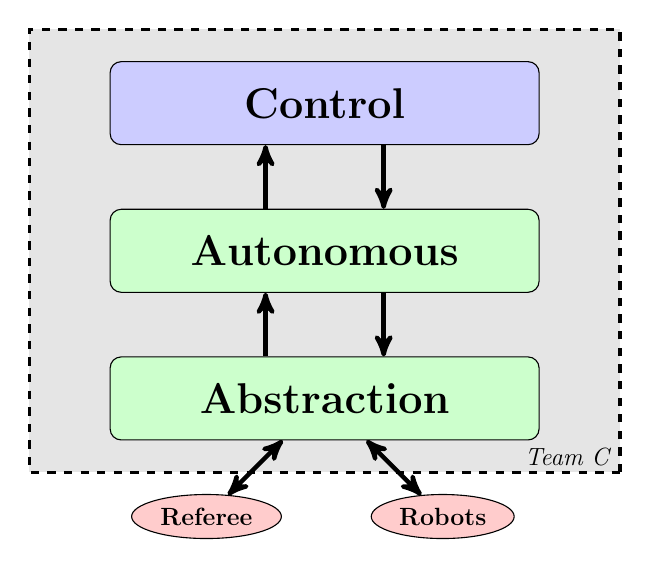
\begin{tikzpicture}[scale=0.75, transform shape]		
		    % Layers
			\node [block] (control) {\huge \textbf{Control}};
		    \node [block-active, below of=control] (autonomous) {\huge \textbf{Autonomous}};
			\node [block-active, below of=autonomous] (abstraction) {\huge \textbf{Abstraction}};
	
			% Clouds
			\node [below of=abstraction, node distance=2cm] (babstraction) {} ;
			\node [cloud, right of=babstraction] (robots) {\large \textbf{Robots}};
			\node [cloud, left of=babstraction] (referee) {\large \textbf{Referee}};
    
			% Connections
			\path [line] ($(control.south) + (1,0)$) -- ($(autonomous.north) + (1,0)$);
			\path [line] ($(autonomous.north) + (-1,0)$) -- ($(control.south) + (-1,0)$);
	
			\path [line] ($(autonomous.south) + (1,0)$) -- ($(abstraction.north) + (1,0)$);
			\path [line] ($(abstraction.north) + (-1,0)$) -- ($(autonomous.south) + (-1,0)$);
	
			\path [dline] (referee) -- (abstraction);
			\path [dline] (robots) -- (abstraction);
	
			% Background Box
			\begin{pgfonlayer}{background}
				\draw [dashed, very thick, fill=black!10] ($(abstraction) +(5,-1.25)$) rectangle ($(control)+(-5,1.25)$);
				\draw ($(abstraction) +(5,-1)$) node [left] {\large \textit{Team C}};
			\end{pgfonlayer}
		\end{tikzpicture}
	\end{center}
\end{frame}

\begin{frame}
	\frametitle{Classes I}
	\begin{center}
		%!tikz editor 1.0
%!tikz source begin
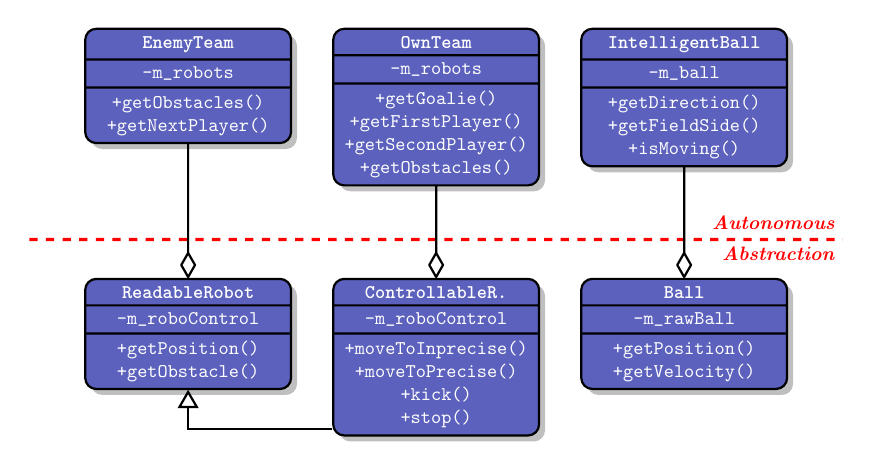
\begin{tikzpicture}[node distance=4.5cm, scale=0.7, transform shape]
	\font\btt=rm-lmtk10
	\definecolor{PresiBlue}{RGB}{50,57,171}
	
	\tikzstyle{class}=[
		rectangle, draw=black, rounded corners, rectangle split, rectangle split parts=3, 
		fill=PresiBlue!80, drop shadow, font=\tt,
        text centered, anchor=north, text=white, text width=3.5cm, thick]
		
	\tikzstyle{inheritance}=[draw, ->, >=open triangle 60, thick]
	\tikzstyle{property}=[draw, <-, >=open diamond, thick]
	\tikzstyle{line}=[-, thick]
   
   % Classes
      
	\node (enemyteam) [class]
	{
		\btt EnemyTeam
		
		\nodepart{second}
		-m\char`_robots
		
		\nodepart{third}
		+getObstacles()\\
		+getNextPlayer()
	};
	
	\node (ownteam) [class, right= of enemyteam.north , anchor=north]
	{
		\btt OwnTeam
		
		\nodepart{second}
		-m\char`_robots
		
		\nodepart{third}
		+getGoalie()\\
		+getFirstPlayer()\\
		+getSecondPlayer()\\
		+getObstacles()
	};
    
	\node (intelligentball) [class, right= of ownteam.north, anchor=north]
	{
		\btt IntelligentBall
		
		\nodepart{second}
		-m\char`_ball
		
		\nodepart{third}
		+getDirection()\\
		+getFieldSide()\\
		+isMoving()
	};
	
	\node (readablerobot) [class, below of=enemyteam]
	{
		\btt ReadableRobot
		
		\nodepart{second}
		-m\char`_roboControl
		
		\nodepart{third}
		+getPosition()\\
		+getObstacle()
	};
		
	\node (controllablerobot) [class, right= of readablerobot.north, anchor=north]
	{
		\btt ControllableR.
		
		\nodepart{second}
		-m\char`_roboControl
		
		\nodepart{third}
		+moveToInprecise()\\
		+moveToPrecise()\\
		+kick()\\
		+stop()
	};
	
	\node (ball) [class, right= of controllablerobot.north, anchor=north]
	{
		\btt Ball
		
		\nodepart{second}
		-m\char`_rawBall
		
		\nodepart{third}
		+getPosition()\\
		+getVelocity()
	};
	
	% Connections
	\path [inheritance] (controllablerobot.west) +(0,-1.3) -| (readablerobot);
	\path [property] (controllablerobot) -- (ownteam);
	\path [property] (readablerobot) -- (enemyteam);
	\path [property] (ball) -- (intelligentball);
	
	% Background Box
	\begin{pgfonlayer}{background}
		\draw [dashed, very thick, red] ($(readablerobot.north west) + (-1,0.7)$) -- ($(ball.north east) + (1,0.7)$);
		\draw ($(ball.north east) + (1,0.45)$) node [left, red] {\textbf{\textit{Abstraction}}};
		\draw ($(ball.north east) + (1,1)$) node [left, red] {\textbf{\textit{Autonomous}}};
	\end{pgfonlayer}

	
\end{tikzpicture}
%!tikz source end

	\end{center}
\end{frame}

\begin{frame}
	\frametitle{Layers}
	\begin{center}
		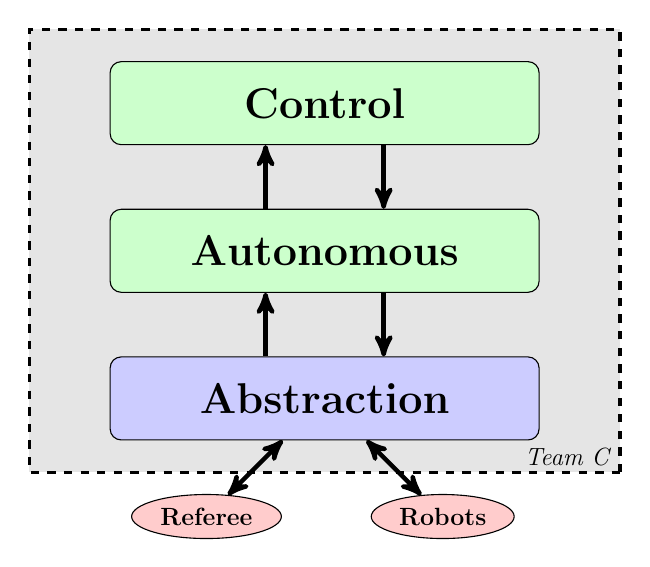
\begin{tikzpicture}[scale=0.75, transform shape]		
		    % Layers
			\node [block-active] (control) {\huge \textbf{Control}};
		    \node [block-active, below of=control] (autonomous) {\huge \textbf{Autonomous}};
			\node [block, below of=autonomous] (abstraction) {\huge \textbf{Abstraction}};
	
			% Clouds
			\node [below of=abstraction, node distance=2cm] (babstraction) {} ;
			\node [cloud, right of=babstraction] (robots) {\large \textbf{Robots}};
			\node [cloud, left of=babstraction] (referee) {\large \textbf{Referee}};
    
			% Connections
			\path [line] ($(control.south) + (1,0)$) -- ($(autonomous.north) + (1,0)$);
			\path [line] ($(autonomous.north) + (-1,0)$) -- ($(control.south) + (-1,0)$);
	
			\path [line] ($(autonomous.south) + (1,0)$) -- ($(abstraction.north) + (1,0)$);
			\path [line] ($(abstraction.north) + (-1,0)$) -- ($(autonomous.south) + (-1,0)$);
	
			\path [dline] (referee) -- (abstraction);
			\path [dline] (robots) -- (abstraction);
	
			% Background Box
			\begin{pgfonlayer}{background}
				\draw [dashed, very thick, fill=black!10] ($(abstraction) +(5,-1.25)$) rectangle ($(control)+(-5,1.25)$);
				\draw ($(abstraction) +(5,-1)$) node [left] {\large \textit{Team C}};
			\end{pgfonlayer}
		\end{tikzpicture}
	\end{center}
\end{frame}

\begin{frame}
	\frametitle{Classes II}
	\center
	%!tikz editor 1.0
%!tikz source begin
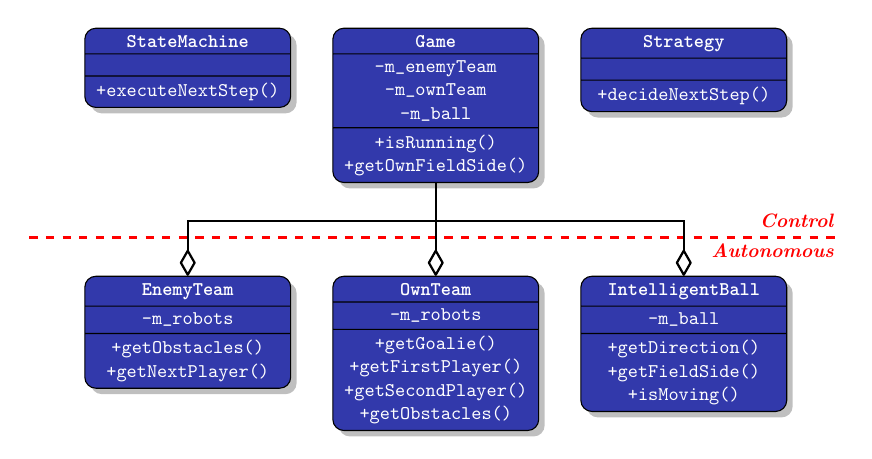
\begin{tikzpicture}[node distance=4.5cm, scale=0.7, transform shape]
	\font\btt=rm-lmtk10
	\definecolor{PresiBlue}{RGB}{50,57,171}
	
	\tikzstyle{class}=[
		rectangle, draw=black, rounded corners, rectangle split, rectangle split parts=3, 
		fill=PresiBlue, drop shadow, font=\tt,
        text centered, anchor=north, text=white, text width=3.5cm]
		
	\tikzstyle{comment}=[
		rectangle, draw=black, rounded corners, fill=green, drop shadow,
        text centered, anchor=north, text=white, text width=3cm]
		
	\tikzstyle{inheritance}=[draw, ->, >=open triangle 60, thick]
	\tikzstyle{property}=[draw, <-, >=open diamond, thick]
	\tikzstyle{line}=[-, thick]
   
   % Classes
      
	\node (enemyteam) [class]
	{
		\btt EnemyTeam
		
		\nodepart{second}
		-m\char`_robots
		
		\nodepart{third}
		+getObstacles()\\
		+getNextPlayer()
	};
	
	\node (ownteam) [class, right= of enemyteam.north , anchor=north]
	{
		\btt OwnTeam
		
		\nodepart{second}
		-m\char`_robots
		
		\nodepart{third}
		+getGoalie()\\
		+getFirstPlayer()\\
		+getSecondPlayer()\\
		+getObstacles()
	};
    
	\node (intelligentball) [class, right= of ownteam.north, anchor=north]
	{
		\btt IntelligentBall
		
		\nodepart{second}
		-m\char`_ball
		
		\nodepart{third}
		+getDirection()\\
		+getFieldSide()\\
		+isMoving()
	};
	
	\node (game) [class, above= of ownteam, anchor=north]
	{
		\btt Game
		
		\nodepart{second}
		-m\char`_enemyTeam\\
		-m\char`_ownTeam\\
		-m\char`_ball\\
		
		\nodepart{third}
		+isRunning()\\
		+getOwnFieldSide()
	};
	
	\node (statemachine) [class, left= of game.north, anchor=north]
	{
		\btt StateMachine
		
		\nodepart{third}
		+executeNextStep()
	};
	
	\node (strategy) [class, right= of game.north, anchor=north]
	{
		\btt Strategy
		
		\nodepart{third}
		+decideNextStep()
	};
	% Connections
	\path [property] (enemyteam.north) -- +(0,1) -| (game.south);
	\path [property] (ownteam.north) -- +(0,1) -| (game.south);
	\path [property] (intelligentball.north) -- +(0,1) -| (game.south);
	
	% Background Box
	\begin{pgfonlayer}{background}
		\draw [dashed, very thick, red] ($(enemyteam.north west) + (-1,0.7)$) -- ($(intelligentball.north east) + (1,0.7)$);
		\draw ($(intelligentball.north east) + (1,0.45)$) node [left, red] {\textbf{\textit{Autonomous}}};
		\draw ($(intelligentball.north east) + (1,1)$) node [left, red] {\textbf{\textit{Control}}};
	\end{pgfonlayer}

	
\end{tikzpicture}
%!tikz source end

\end{frame}

\section{State Machine} 
\begin{frame}
	\frametitle{State Machine - Overview} 	
	\fontsize{6pt}{7.2}\selectfont
	\begin{center}
		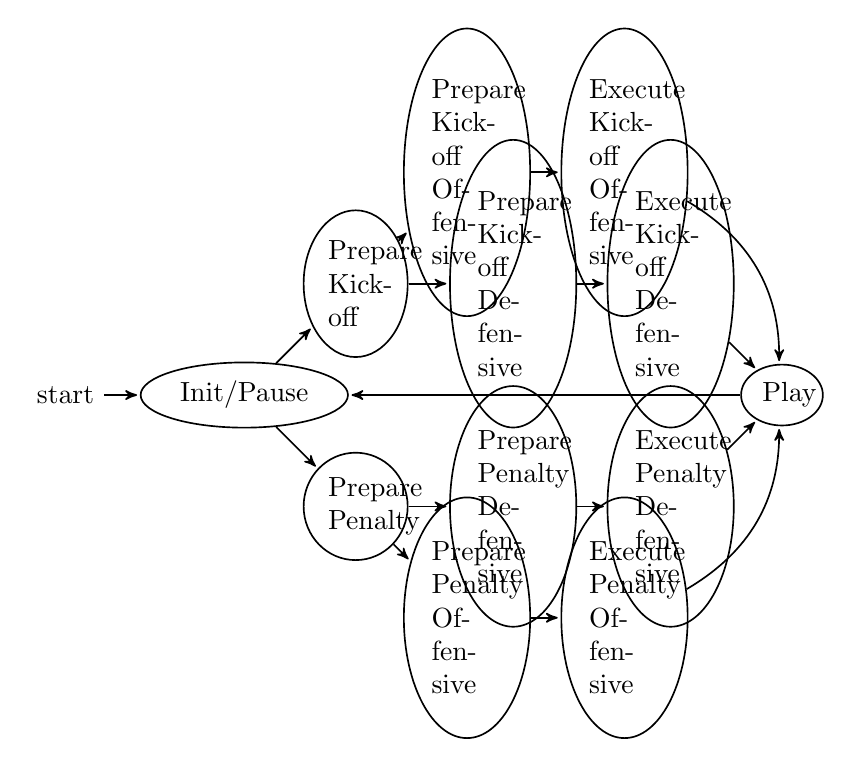
\begin{tikzpicture}[->,>=stealth',shorten >=1pt,auto,node distance=2cm,semithick]
			\tikzstyle{every state}=[draw=none,text=black]
			\tikzset{elliptic state/.style={draw,ellipse}}
			
			\node[initial,elliptic state] (init)                    {Init/Pause};
			\node[elliptic state]         (prepareKickOff) [above right of=init,text width=0.7cm] {Prepare Kickoff};
			\node[elliptic state]         (prepareKickOffOffensive) [above right of=prepareKickOff,text width=0.9cm] {Prepare Kickoff Offensive};
			\node[elliptic state]         (executeKickOffOffensive) [right of=prepareKickOffOffensive,text width=0.9cm] {Execute Kickoff Offensive};
			\node[elliptic state]         (prepareKickOffDefensive) [right of=prepareKickOff,text width=0.9cm]       {Prepare Kickoff Defensive};
			\node[elliptic state]         (executeKickOffDefensive) [right of=prepareKickOffDefensive,text width=0.9cm]       {Execute Kickoff Defensive};
			\node[elliptic state]         (preparePenalty) [below right of=init,text width=0.7cm] {Prepare Penalty};
			\node[elliptic state]         (preparePenaltyOffensive) [below right of=preparePenalty,text width=0.9cm] {Prepare Penalty Offensive};
			\node[elliptic state]         (executePenaltyOffensive) [right of=preparePenaltyOffensive,text width=0.9cm] {Execute Penalty Offensive};
			\node[elliptic state]         (preparePenaltyDefensive) [right of=preparePenalty,text width=0.9cm]       {Prepare Penalty Defensive};
			\node[elliptic state]         (executePenaltyDefensive) [right of=preparePenaltyDefensive,text width=0.9cm]       {Execute Penalty Defensive};
			\node[elliptic state]         (play) [below right of=executeKickOffDefensive,text width=0.5cm]       {Play};
			
			\path (init) 
						edge (prepareKickOff)
			  			edge (preparePenalty)
			      (prepareKickOff) 
			        	edge (prepareKickOffOffensive)
			            edge (prepareKickOffDefensive)
			      (prepareKickOffOffensive)
			        	edge (executeKickOffOffensive)
			      (prepareKickOffDefensive)
			        	edge (executeKickOffDefensive)
			      (executeKickOffOffensive)
				       	edge [bend left] (play)
			      (executeKickOffDefensive)
			        	edge (play)
			      (preparePenalty) 
			        	edge (preparePenaltyOffensive)
			            edge (preparePenaltyDefensive)
			      (preparePenaltyOffensive)
			        	edge (executePenaltyOffensive)
			      (preparePenaltyDefensive)
			        	edge (executePenaltyDefensive)
			      (executePenaltyOffensive)
			        	edge [bend right] (play)
			      (executePenaltyDefensive)
			        	edge (play)
			      (play)
			        	edge (init);
		\end{tikzpicture}
	\end{center}
\end{frame}

\begin{frame}
	\frametitle{Init/Pause} 	
	\fontsize{6pt}{7.2}\selectfont
	\begin{center}
		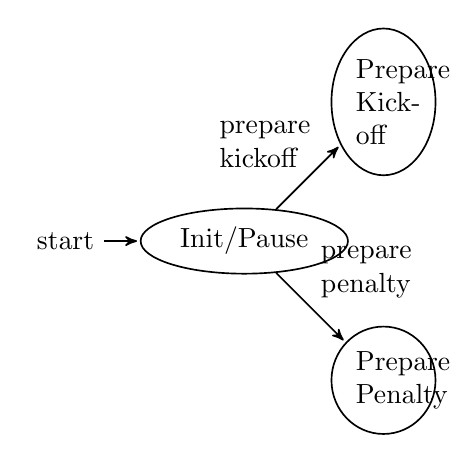
\begin{tikzpicture}[->,>=stealth',shorten >=1pt,auto,node distance=2.5cm,semithick]
			\tikzstyle{every state}=[draw=none,text=black]
			\tikzset{elliptic state/.style={draw,ellipse}}
			
			\node[initial,elliptic state] (init)                    {Init/Pause};
			\node[elliptic state]         (prepareKickOff) [above right of=init,text width=0.7cm] {Prepare Kickoff};
			\node[elliptic state]         (preparePenalty) [below right of=init,text width=0.7cm] {Prepare Penalty};
			
			\path (init) 
						edge node[text width=1cm]{prepare kickoff} (prepareKickOff)
			  			edge node[text width=1cm]{prepare penalty} (preparePenalty);
		\end{tikzpicture}
	\end{center}
\end{frame}

\begin{frame}
	\frametitle{Kickoff} 	
	\fontsize{6pt}{7.2}\selectfont
	\begin{center}
		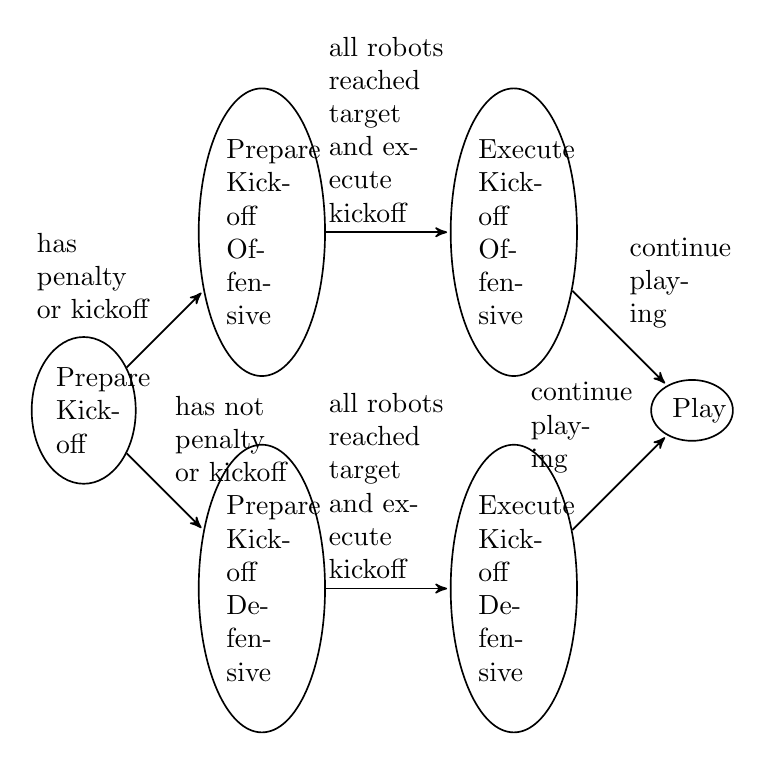
\begin{tikzpicture}[->,>=stealth',shorten >=1pt,auto,node distance=3.2cm,semithick]
			\tikzstyle{every state}=[draw=none,text=black]
			\tikzset{elliptic state/.style={draw,ellipse}}
			
			\node[elliptic state]         (prepareKickOff) [text width=0.7cm] {Prepare Kickoff};
			\node[elliptic state]         (prepareKickOffOffensive) [above right of=prepareKickOff,text width=0.9cm] {Prepare Kickoff Offensive};
			\node[elliptic state]         (executeKickOffOffensive) [right of=prepareKickOffOffensive,text width=0.9cm] {Execute Kickoff Offensive};
			\node[elliptic state]         (prepareKickOffDefensive) [below right of=prepareKickOff,text width=0.9cm]       {Prepare Kickoff Defensive};
			\node[elliptic state]         (executeKickOffDefensive) [right of=prepareKickOffDefensive,text width=0.9cm]       {Execute Kickoff Defensive};
			\node[elliptic state]         (play) [above right of=executeKickOffDefensive,text width=0.5cm]       {Play};
			
			\path (prepareKickOff) 
			        	edge node[text width=1.5cm]{has penalty or kickoff} (prepareKickOffOffensive)
			            edge node[text width=1.5cm]{has not penalty or kickoff} (prepareKickOffDefensive)
			      (prepareKickOffOffensive)
			        	edge node[text width=1.5cm]{all robots reached target and execute kickoff} (executeKickOffOffensive)
			      (prepareKickOffDefensive)
			        	edge node[text width=1.5cm]{all robots reached target and execute kickoff} (executeKickOffDefensive)
			      (executeKickOffOffensive)
				       	edge node[text width=1cm]{continue playing} (play)
			      (executeKickOffDefensive)
			        	edge node[text width=1cm]{continue playing} (play);
		\end{tikzpicture}
	\end{center}
\end{frame}

\begin{frame}
	\frametitle{Penalty} 	
	\fontsize{6pt}{7.2}\selectfont
	\begin{center}
		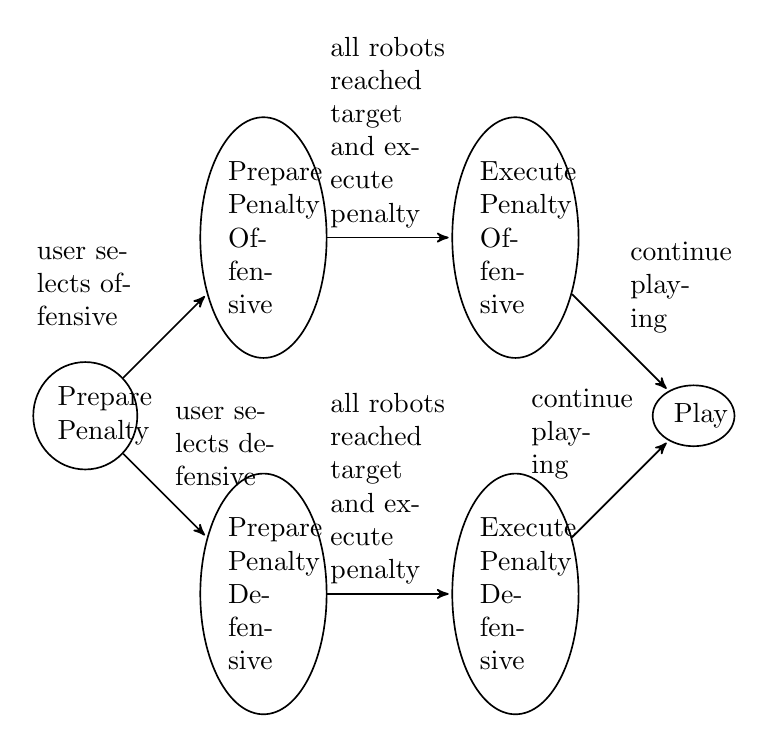
\begin{tikzpicture}[->,>=stealth',shorten >=1pt,auto,node distance=3.2cm,semithick]
			\tikzstyle{every state}=[draw=none,text=black]
			\tikzset{elliptic state/.style={draw,ellipse}}
			
			\node[elliptic state]         (preparePenalty) [text width=0.7cm] {Prepare Penalty};
			\node[elliptic state]         (preparePenaltyOffensive) [above right of=preparePenalty,text width=0.9cm] {Prepare Penalty Offensive};
			\node[elliptic state]         (executePenaltyOffensive) [right of=preparePenaltyOffensive,text width=0.9cm] {Execute Penalty Offensive};
			\node[elliptic state]         (preparePenaltyDefensive) [below right of=preparePenalty,text width=0.9cm]       {Prepare Penalty Defensive};
			\node[elliptic state]         (executePenaltyDefensive) [right of=preparePenaltyDefensive,text width=0.9cm]       {Execute Penalty Defensive};
			\node[elliptic state]         (play) [above right of=executePenaltyDefensive,text width=0.5cm]       {Play};
			
			\path (preparePenalty) 
			        	edge node[text width=1.5cm]{user selects offensive} (preparePenaltyOffensive)
			            edge node[text width=1.5cm]{user selects defensive} (preparePenaltyDefensive)
			      (preparePenaltyOffensive)
			        	edge node[text width=1.5cm]{all robots reached target and execute penalty} (executePenaltyOffensive)
			      (preparePenaltyDefensive)
			        	edge node[text width=1.5cm]{all robots reached target and execute penalty} (executePenaltyDefensive)
			      (executePenaltyOffensive)
				       	edge node[text width=1cm]{continue playing} (play)
			      (executePenaltyDefensive)
			        	edge node[text width=1cm]{continue playing} (play);
		\end{tikzpicture}
	\end{center}
\end{frame}

\section{Control} 
\begin{frame}
	\frametitle{Control I}	
	\begin{figure}
		\centering
		\begin{overpic}[width=0.8\textwidth]{roboline.pdf}
			\put(10,39){\small Start}
			\put(10,44){\small Goal}
			\put(15,7){\small \color{blue} d}
	   	\end{overpic}
	\end{figure}	
\end{frame}

\begin{frame}
	\frametitle{Control II}
	\begin{figure}
		\centering
		\begin{overpic}[width=0.8\textwidth]{control.pdf}
			\put(30,15){\textsc{PI}}
			\put(30,29){\textsc{PI}}
			\put(10.5,15.5){\tiny +}
			\put(10.5,29.75){\tiny +}
			\put(57.15,29.75){\tiny +}
			\put(73,28){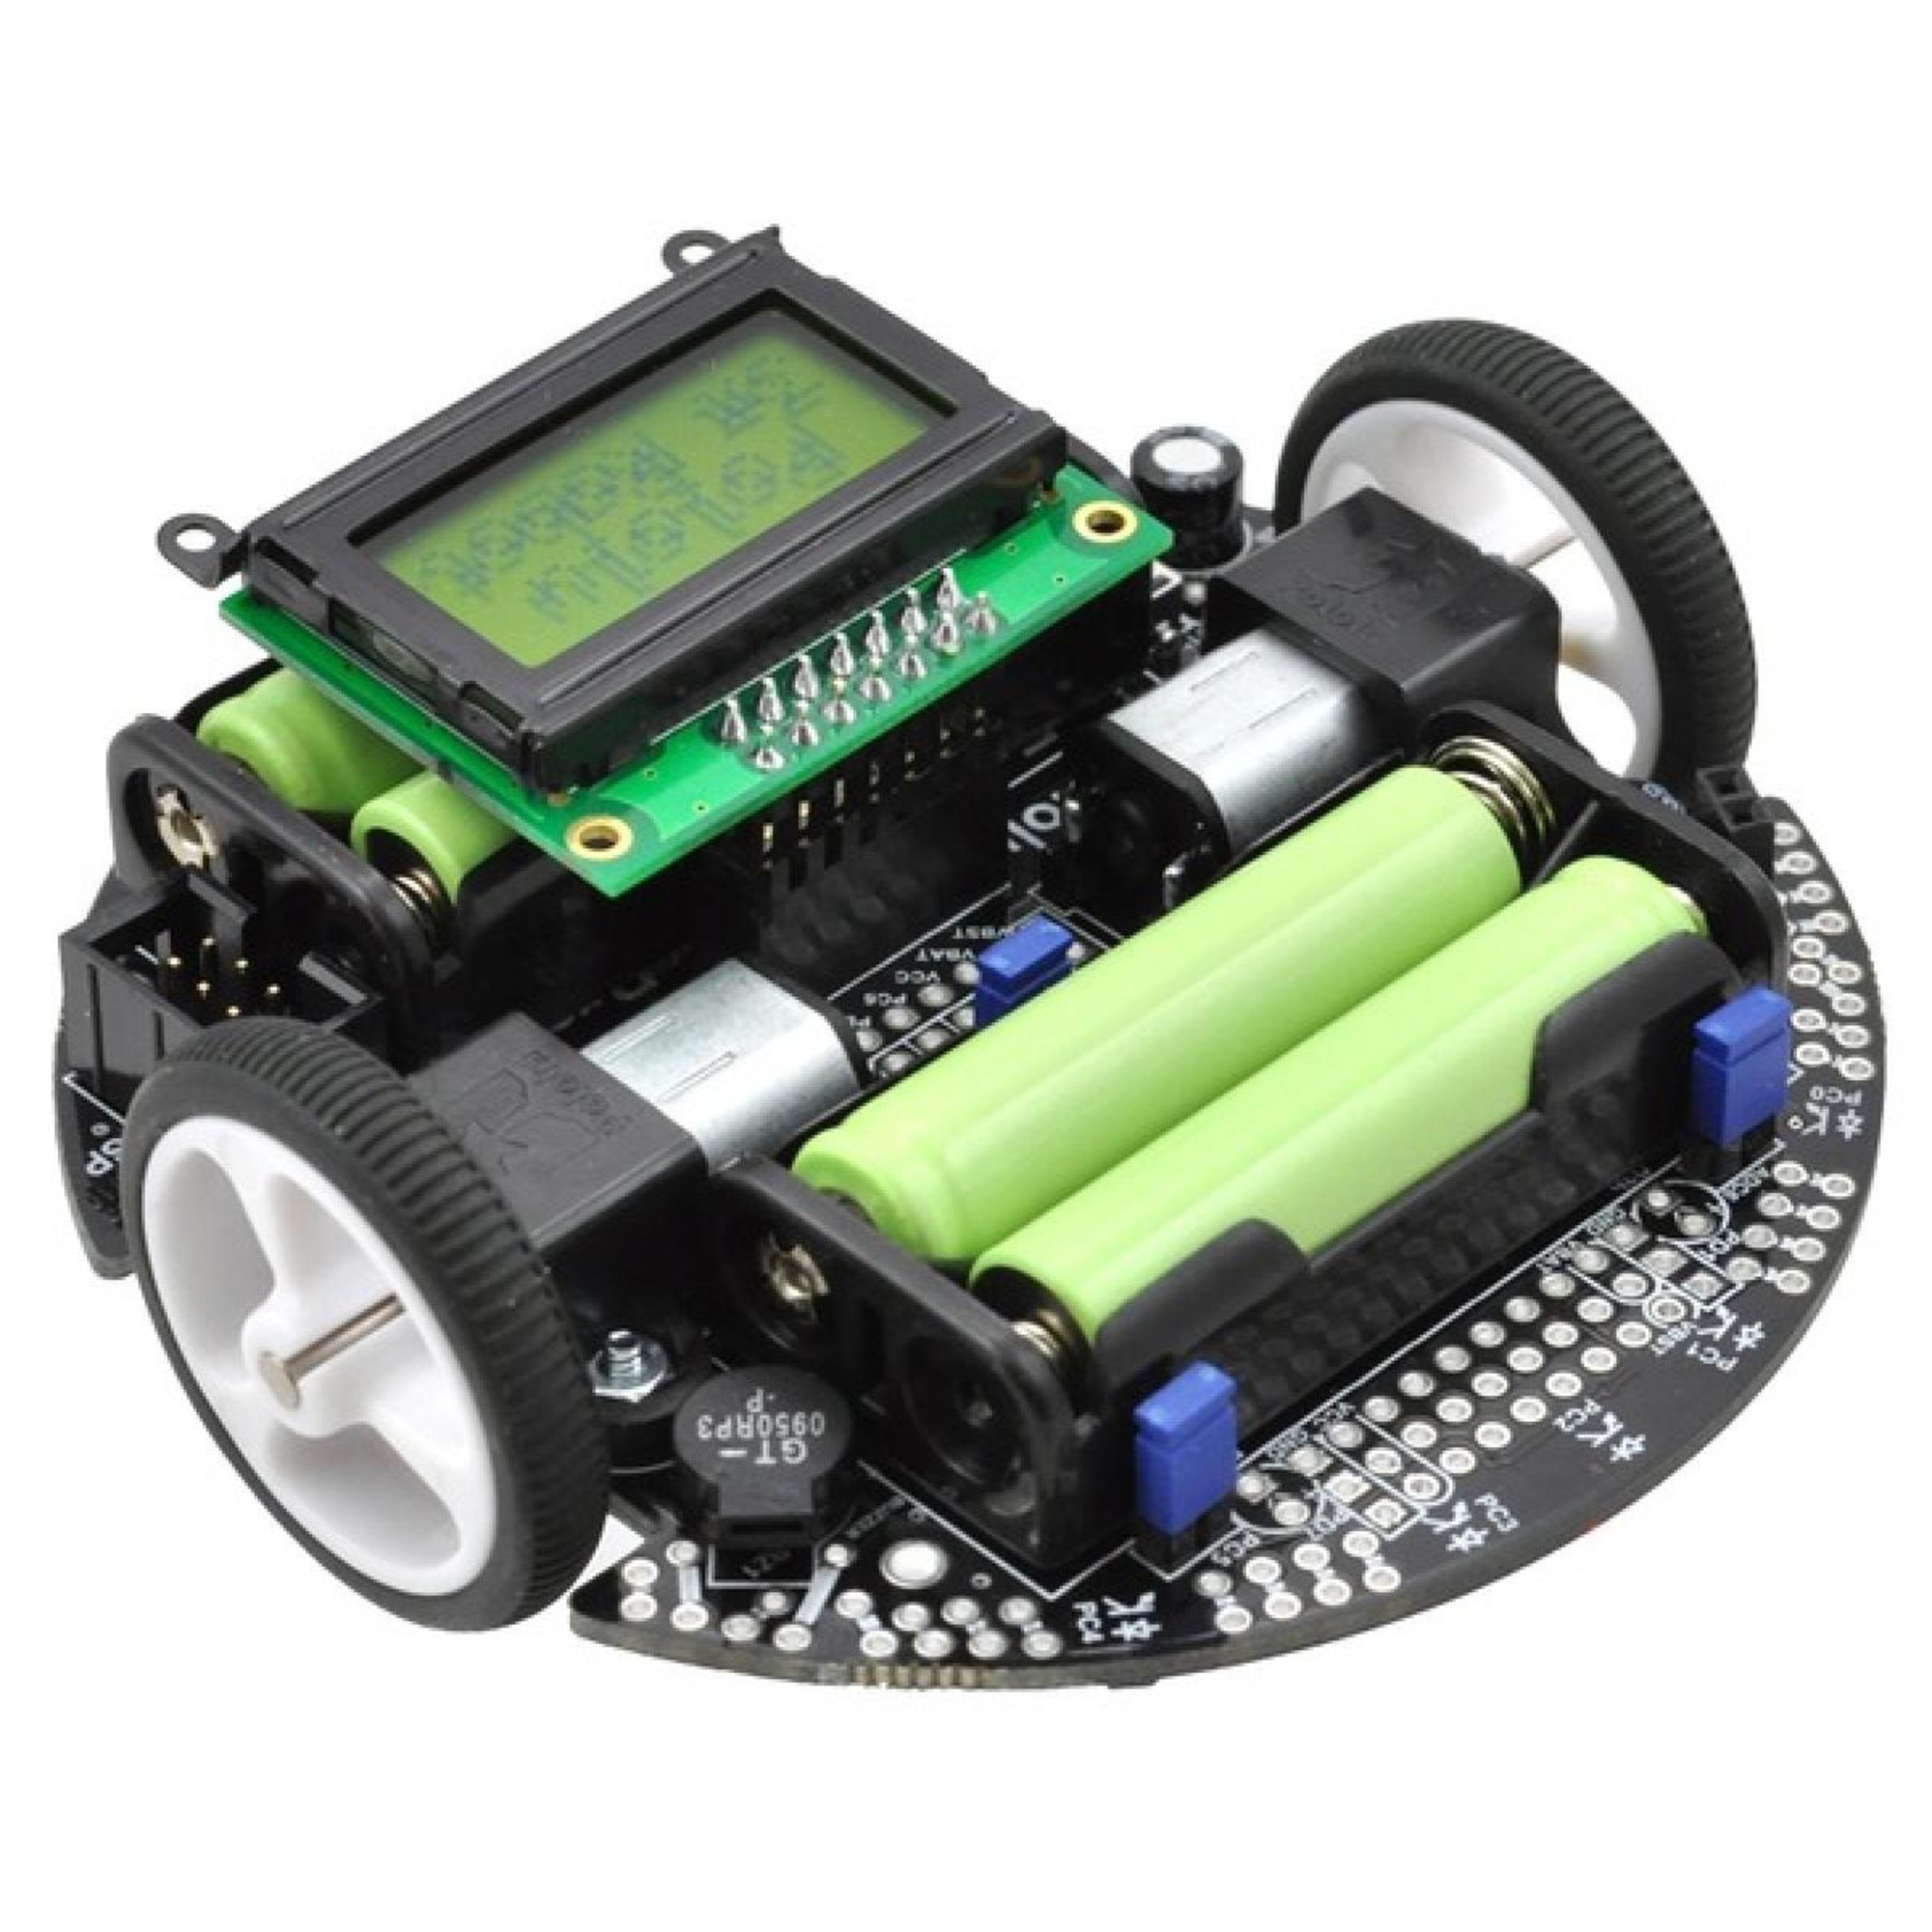
\includegraphics[scale=0.02]{3pi.pdf}}
			\put(73,25.5){\tiny Tracker}
			\put(86,32){\tiny $\left[\mathbf{x},\Omega \right]$}
			\put(60,43.5){\tiny $\Vert \mathbf{x} - \mathbf{x}_\mathrm{g} \Vert_2$}
			\put(65,1.5){\scriptsize $d$}
			\put(43,29){\scriptsize $>60$}
			\put(-3,29){\small $0$}
			\put(-3,15){\small $0$}
	   	\end{overpic}
	\end{figure}	
\end{frame}

\section{Collision Avoidance} 
\begin{frame}
	\frametitle{Collision Avoidance}
	\begin{itemize}
		\item no direct collision avoidance
		\item Router
		\begin{itemize}
			\item calculates only save routes
			\item route ...
		\end{itemize}
	\end{itemize}
\end{frame}

\begin{frame}
	\frametitle{Router} 
	\begin{center}
		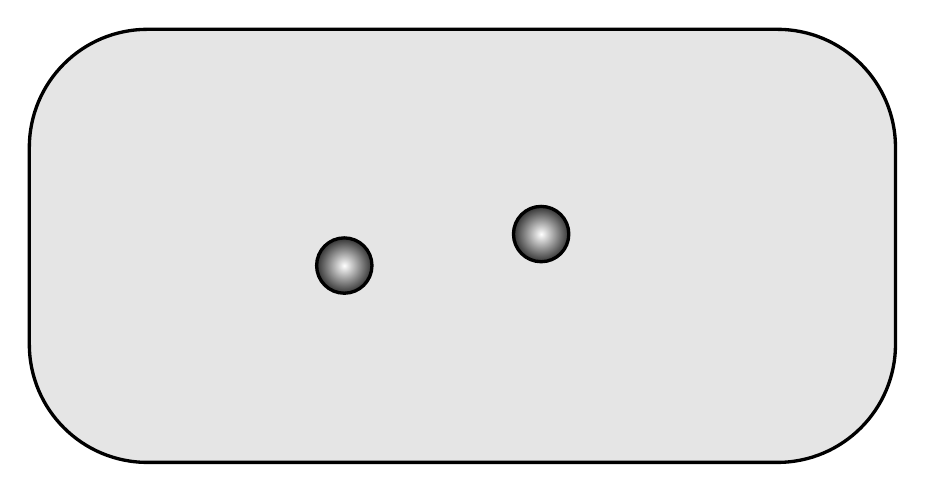
\begin{tikzpicture}
			% Background Box
			\begin{pgfonlayer}{background}
				\draw [rounded corners=1.5cm, very thick, fill=black!10] (-2.5,-3) rectangle (8.5,2.5);
			\end{pgfonlayer}
			% Folie 1
			\robot at (0,0) {};
			\node[obstacle] at (1.5,-.5) {}; 
			\node[obstacle] at (4,-0.1) {};
			\goal at (6,0) {}; 
		\end{tikzpicture}
	\end{center}		
\end{frame}

\begin{frame}
	\frametitle{Router} 
	\begin{center}
		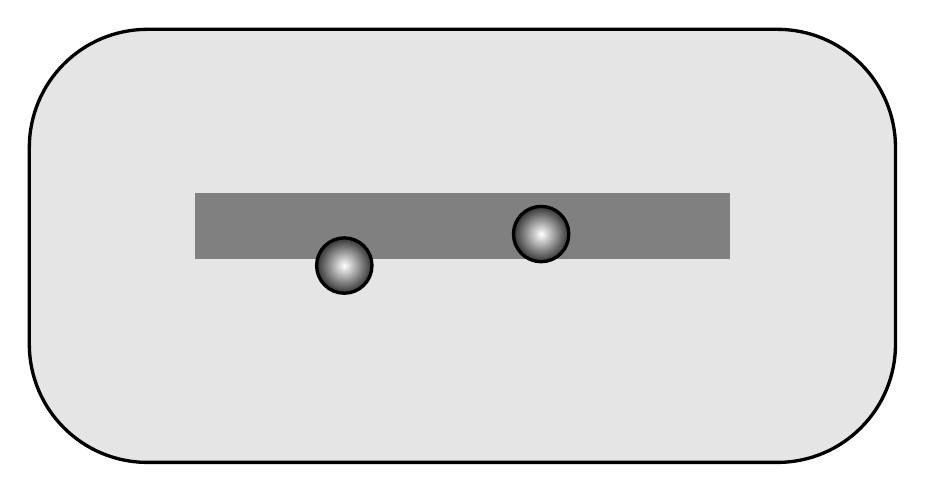
\begin{tikzpicture}
			% Background Box
			\begin{pgfonlayer}{background}
				\draw [rounded corners=1.5cm, very thick, fill=black!10] (-2.5,-3) rectangle (8.5,2.5);
			\end{pgfonlayer}
			% Folie 2
			\path[edge] (-0.4,0) -- (6.4,0);
			\robot at (0,0) {};
			\node[obstacle] at (1.5,-.5) {}; 
			\node[obstacle] at (4,-0.1) {};
			\goal at (6,0) {};
		\end{tikzpicture}
	\end{center}	
\end{frame}

\begin{frame}
	\frametitle{Router} 
	\begin{center}
		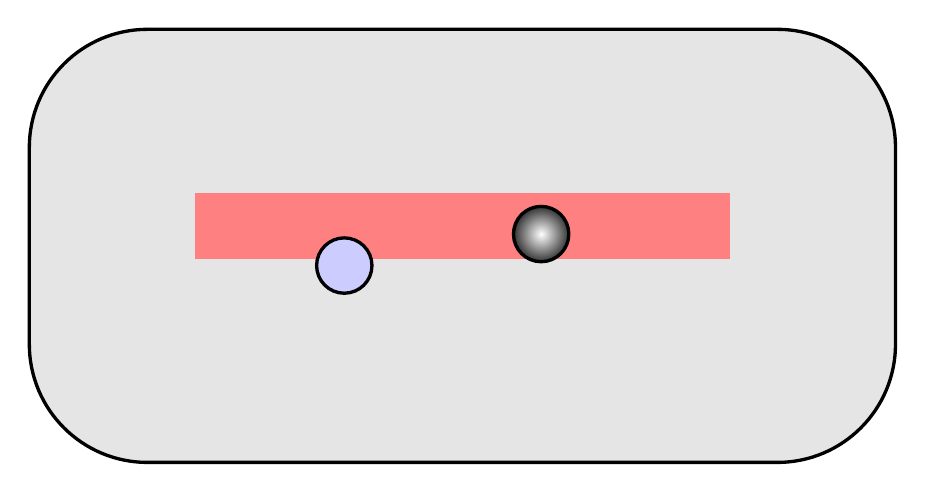
\begin{tikzpicture}
			% Background Box
			\begin{pgfonlayer}{background}
				\draw [rounded corners=1.5cm, very thick, fill=black!10] (-2.5,-3) rectangle (8.5,2.5);
			\end{pgfonlayer}
			% Folie 3
			\path[ignored edge] (-0.4,0) -- (6.4,0);
			\robot at (0,0) {};
			\node[selected obstacle] at (1.5,-.5) {}; 
			\node[obstacle] at (4,-0.1) {};
			\goal at (6,0) {};
			\goalHelp at (1.5,.5) {};
			\goalHelp at (1.5,-1.8) {};
		\end{tikzpicture}
	\end{center}	
\end{frame}

\begin{frame}
	\frametitle{Router} 
	\begin{center}
		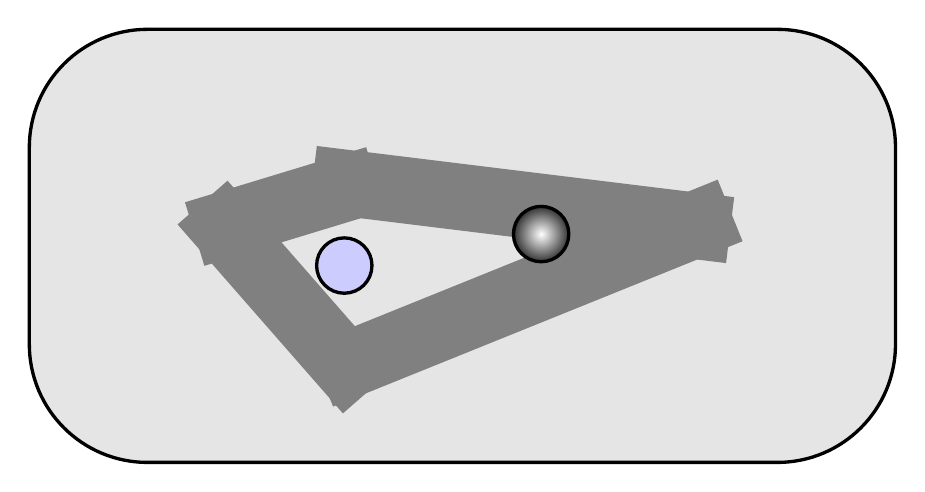
\begin{tikzpicture}
			% Background Box
			\begin{pgfonlayer}{background}
				\draw [rounded corners=1.5cm, very thick, fill=black!10] (-2.5,-3) rectangle (8.5,2.5);
			\end{pgfonlayer}
			% Folie 4
			\path[edge] (-0.4,-0.1) -- (1.9,0.6);
			\path[edge] (-0.3,0.3) -- (1.8,-2.1);
			\path[edge] (1.1,0.6) -- (6.4,-0.05);
			\path[edge] (1.2,-1.9) -- (6.4,0.2);
			\robot at (0,0) {};
			\node[selected obstacle] at (1.5,-.5) {}; 
			\node[obstacle] at (4,-0.1) {};
			\goal at (6,0) {};
			\goalHelp at (1.5,.5) {};
			\goalHelp at (1.5,-1.8) {};
		\end{tikzpicture}
	\end{center}	
\end{frame}

\begin{frame}
	\frametitle{Router} 
	\begin{center}
		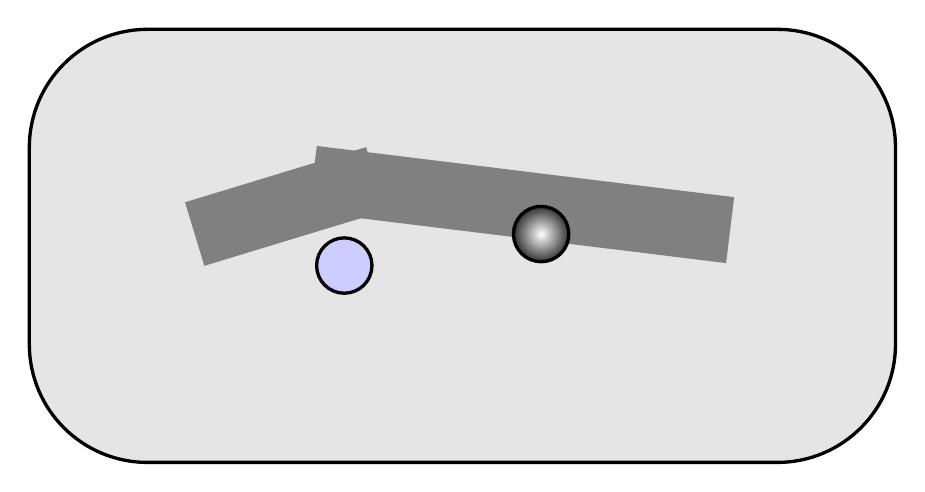
\begin{tikzpicture}
			% Background Box
			\begin{pgfonlayer}{background}
				\draw [rounded corners=1.5cm, very thick, fill=black!10] (-2.5,-3) rectangle (8.5,2.5);
			\end{pgfonlayer}
			% Folie 5
			\path[edge] (-0.4,-0.1) -- (1.9,0.6);
			\path[edge] (1.1,0.6) -- (6.4,-0.05);
			\robot at (0,0) {};
			\node[selected obstacle] at (1.5,-.5) {}; 
			\node[obstacle] at (4,-0.1) {};
			\goal at (6,0) {};
			\goalHelp at (1.5,.5) {};
		\end{tikzpicture}
	\end{center}	
\end{frame}

\begin{frame}
	\frametitle{Router} 
	\begin{center}
		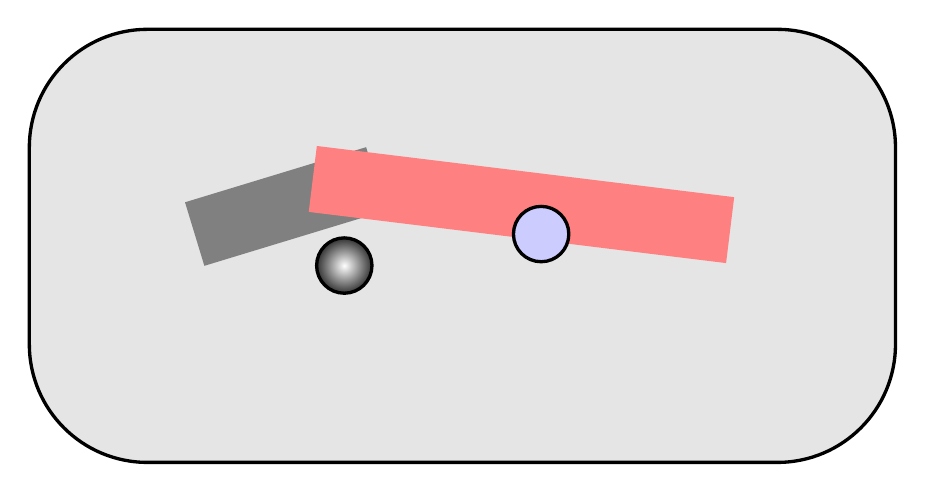
\begin{tikzpicture}
			% Background Box
			\begin{pgfonlayer}{background}
				\draw [rounded corners=1.5cm, very thick, fill=black!10] (-2.5,-3) rectangle (8.5,2.5);
			\end{pgfonlayer}
			% Folie 6
			\path[edge] (-0.4,-0.1) -- (1.9,0.6);
			\path[ignored edge] (1.1,0.6) -- (6.4,-0.05);
			\robot at (0,0) {};
			\node[obstacle] at (1.5,-.5) {}; 
			\node[selected obstacle] at (4,-0.1) {};
			\goal at (6,0) {};
			\goalHelp at (1.5,.5) {};
			\goalHelp at (4,.9) {};
			\goalHelp at (4,-1.1) {};
		\end{tikzpicture}
	\end{center}	
\end{frame}

\begin{frame}
	\frametitle{Router} 
	\begin{center}
		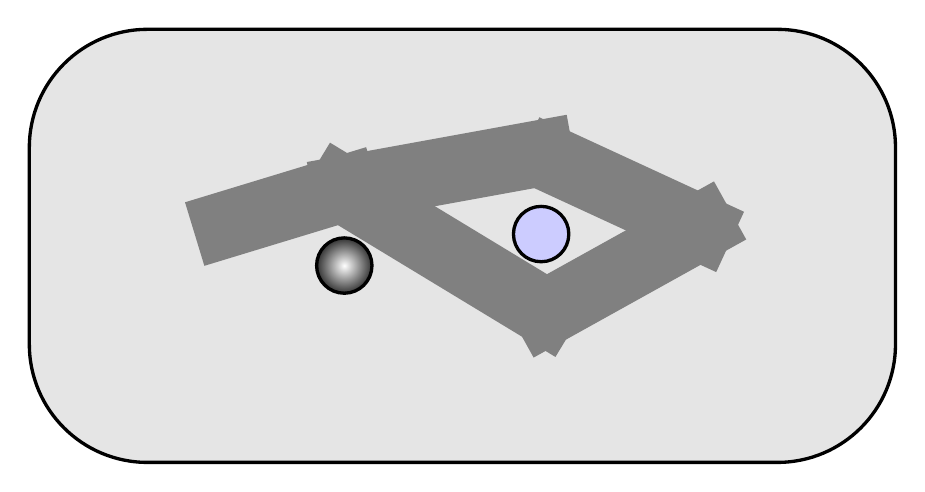
\begin{tikzpicture}
			% Background Box
			\begin{pgfonlayer}{background}
				\draw [rounded corners=1.5cm, very thick, fill=black!10] (-2.5,-3) rectangle (8.5,2.5);
			\end{pgfonlayer}
			% Folie 7
			\path[edge] (-0.4,-0.1) -- (1.9,0.6);
			\path[edge] (1.1,0.7) -- (4.4,-1.3);
			\path[edge] (1.1,0.4) -- (4.4,1);
			\path[edge] (3.7,-1.3) -- (6.4,0.2);
			\path[edge] (3.8,1) -- (6.4,-0.2);
			\robot at (0,0) {};
			\node[obstacle] at (1.5,-.5) {}; 
			\node[selected obstacle] at (4,-0.1) {};
			\goal at (6,0) {};
			\goalHelp at (1.5,.5) {};
			\goalHelp at (4,.9) {};
			\goalHelp at (4,-1.1) {};
		\end{tikzpicture}
	\end{center}	
\end{frame}

\begin{frame}
	\frametitle{Router} 
	\begin{center}
		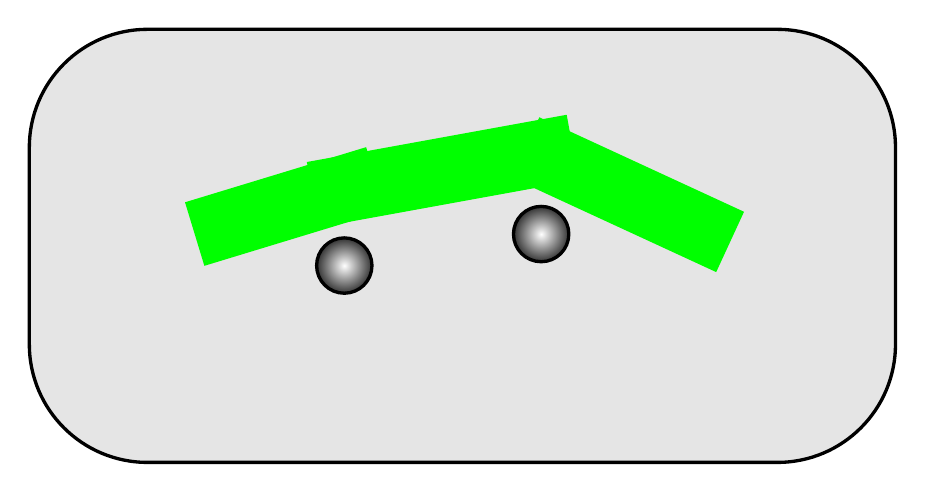
\begin{tikzpicture}
			% Background Box
			\begin{pgfonlayer}{background}
				\draw [rounded corners=1.5cm, very thick, fill=black!10] (-2.5,-3) rectangle (8.5,2.5);
			\end{pgfonlayer}
			% Folie 8
			\path[selected edge] (-0.4,-0.1) -- (1.9,0.6);
			\path[selected edge] (1.1,0.4) -- (4.4,1);
			\path[selected edge] (3.8,1) -- (6.4,-0.2);
			\robot at (0,0) {};
			\node[obstacle] at (1.5,-.5) {}; 
			\node[obstacle] at (4,-0.1) {};
			\goal at (6,0) {};
			\goalHelp at (1.5,.5) {};
			\goalHelp at (4,.9) {};
		\end{tikzpicture}
	\end{center}	
\end{frame}

\section{Gantt Chart} 
\begin{frame}
	\frametitle{Gantt chart} 
\end{frame}

\section{}
\begin{frame}
	\hfill
	\begin{beamercolorbox}[shadow=true, rounded=true, wd=10cm]{presinative}
		\centering
		\Large{\textbf{Thank you for your attention!}}
	\end{beamercolorbox}
	\hfill
\end{frame}

\end{document}

